\documentclass{extbook}[14pt]
\usepackage{multicol, enumerate, enumitem, hyperref, color, soul, setspace, parskip, fancyhdr, amssymb, amsthm, amsmath, bbm, latexsym, units, mathtools}
\everymath{\displaystyle}
\usepackage[headsep=0.5cm,headheight=0cm, left=1 in,right= 1 in,top= 1 in,bottom= 1 in]{geometry}
\usepackage{dashrule}  % Package to use the command below to create lines between items
\newcommand{\litem}[1]{\item #1

\rule{\textwidth}{0.4pt}}
\pagestyle{fancy}
\lhead{}
\chead{Answer Key for Makeup Progress Quiz -1 Version C}
\rhead{}
\lfoot{7547-2949}
\cfoot{}
\rfoot{Fall 2020}
\begin{document}
\textbf{This key should allow you to understand why you choose the option you did (beyond just getting a question right or wrong). \href{https://xronos.clas.ufl.edu/mac1105spring2020/courseDescriptionAndMisc/Exams/LearningFromResults}{More instructions on how to use this key can be found here}.}

\textbf{If you have a suggestion to make the keys better, \href{https://forms.gle/CZkbZmPbC9XALEE88}{please fill out the short survey here}.}

\textit{Note: This key is auto-generated and may contain issues and/or errors. The keys are reviewed after each exam to ensure grading is done accurately. If there are issues (like duplicate options), they are noted in the offline gradebook. The keys are a work-in-progress to give students as many resources to improve as possible.}

\rule{\textwidth}{0.4pt}

\begin{enumerate}\litem{
Describe the end behavior of the polynomial below.
\[ f(x) = 9(x + 2)^{4}(x - 2)^{9}(x - 9)^{3}(x + 9)^{5} \]

The solution is the graph below, which is option D.
\begin{center}
    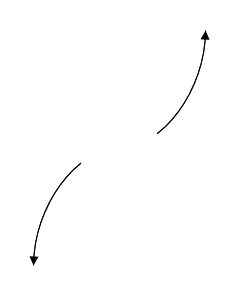
\includegraphics[width=0.3\textwidth]{../Figures/polyEndBehaviorDC.png}
\end{center}\begin{enumerate}[label=\Alph*.]
\begin{multicols}{2}
\item 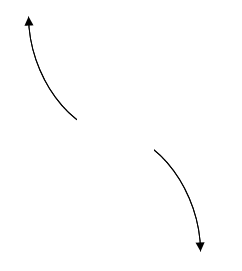
\includegraphics[width = 0.3\textwidth]{../Figures/polyEndBehaviorAC.png}
\item 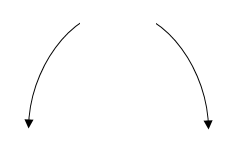
\includegraphics[width = 0.3\textwidth]{../Figures/polyEndBehaviorBC.png}
\item 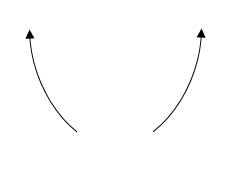
\includegraphics[width = 0.3\textwidth]{../Figures/polyEndBehaviorCC.png}
\item 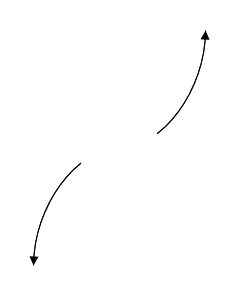
\includegraphics[width = 0.3\textwidth]{../Figures/polyEndBehaviorDC.png}
\end{multicols}\item None of the above.\end{enumerate}
\textbf{General Comment:} Remember that end behavior is determined by the leading coefficient AND whether the \textbf{sum} of the multiplicities is positive or negative.
}
\litem{
Describe the zero behavior of the zero $x = 8$ of the polynomial below.
\[ f(x) = 8(x + 8)^{7}(x - 8)^{12}(x - 4)^{4}(x + 4)^{8} \]

The solution is the graph below, which is option C.
\begin{center}
    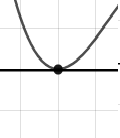
\includegraphics[width=0.3\textwidth]{../Figures/polyZeroBehaviorCopyCC.png}
\end{center}\begin{enumerate}[label=\Alph*.]
\begin{multicols}{2}
\item 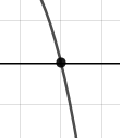
\includegraphics[width = 0.3\textwidth]{../Figures/polyZeroBehaviorCopyAC.png}
\item 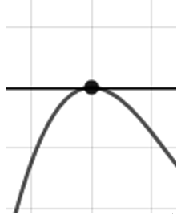
\includegraphics[width = 0.3\textwidth]{../Figures/polyZeroBehaviorCopyBC.png}
\item 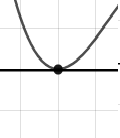
\includegraphics[width = 0.3\textwidth]{../Figures/polyZeroBehaviorCopyCC.png}
\item 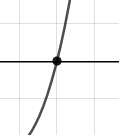
\includegraphics[width = 0.3\textwidth]{../Figures/polyZeroBehaviorCopyDC.png}
\end{multicols}\item None of the above.\end{enumerate}
\textbf{General Comment:} You will need to sketch the entire graph, then zoom in on the zero the question asks about.
}
\litem{
Construct the lowest-degree polynomial given the zeros below. Then, choose the intervals that contain the coefficients of the polynomial in the form $x^3+bx^2+cx+d$.
\[ -4 + 2 i \text{ and } 1 \]

The solution is \( x^{3} +7 x^{2} +12 x -20 \), which is option A.\begin{enumerate}[label=\Alph*.]
\item \( b \in [5, 17], c \in [12, 13], \text{ and } d \in [-24, -17] \)

* $x^{3} +7 x^{2} +12 x -20$, which is the correct option.
\item \( b \in [-6, 2], c \in [-2, 6], \text{ and } d \in [-5, -2] \)

$x^{3} + x^{2} +3 x -4$, which corresponds to multiplying out $(x + 4)(x -1)$.
\item \( b \in [-13, -1], c \in [12, 13], \text{ and } d \in [19, 24] \)

$x^{3} -7 x^{2} +12 x + 20$, which corresponds to multiplying out $(x-(-4 + 2 i))(x-(-4 - 2 i))(x + 1)$.
\item \( b \in [-6, 2], c \in [-4, 0], \text{ and } d \in [-1, 7] \)

$x^{3} + x^{2} -3 x + 2$, which corresponds to multiplying out $(x -2)(x -1)$.
\item \( \text{None of the above.} \)

This corresponds to making an unanticipated error or not understanding how to use nonreal complex numbers to create the lowest-degree polynomial. If you chose this and are not sure what you did wrong, please contact the coordinator for help.
\end{enumerate}

\textbf{General Comment:} Remember that the conjugate of $a+bi$ is $a-bi$. Since these zeros always come in pairs, we need to multiply out $(x-(-4 + 2 i))(x-(-4 - 2 i))(x-(1))$.
}
\litem{
Describe the zero behavior of the zero $x = -5$ of the polynomial below.
\[ f(x) = 6(x + 4)^{12}(x - 4)^{9}(x - 5)^{5}(x + 5)^{2} \]

The solution is the graph below, which is option C.
\begin{center}
    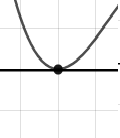
\includegraphics[width=0.3\textwidth]{../Figures/polyZeroBehaviorCC.png}
\end{center}\begin{enumerate}[label=\Alph*.]
\begin{multicols}{2}
\item 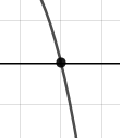
\includegraphics[width = 0.3\textwidth]{../Figures/polyZeroBehaviorAC.png}
\item 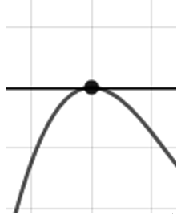
\includegraphics[width = 0.3\textwidth]{../Figures/polyZeroBehaviorBC.png}
\item 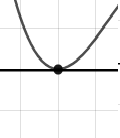
\includegraphics[width = 0.3\textwidth]{../Figures/polyZeroBehaviorCC.png}
\item 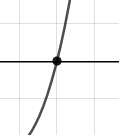
\includegraphics[width = 0.3\textwidth]{../Figures/polyZeroBehaviorDC.png}
\end{multicols}\item None of the above.\end{enumerate}
\textbf{General Comment:} You will need to sketch the entire graph, then zoom in on the zero the question asks about.
}
\litem{
Which of the following equations \textit{could} be of the graph presented below?

\begin{center}
    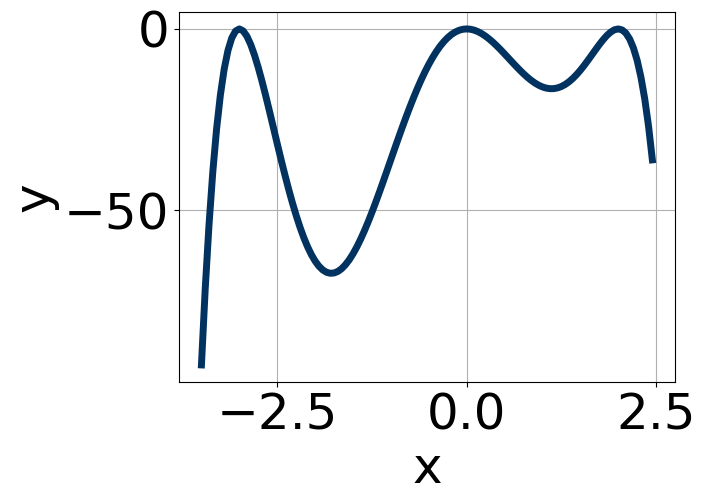
\includegraphics[width=0.5\textwidth]{../Figures/polyGraphToFunctionCopyC.png}
\end{center}




The solution is \( -12x^{6} (x + 3)^{6} (x - 2)^{10} \), which is option E.\begin{enumerate}[label=\Alph*.]
\item \( 16x^{10} (x + 3)^{10} (x - 2)^{5} \)

The factor $(x - 2)$ should have an even power and the leading coefficient should be the opposite sign.
\item \( -8x^{9} (x + 3)^{8} (x - 2)^{5} \)

The factors $x$ and $(x - 2)$ should both have even powers.
\item \( -19x^{4} (x + 3)^{10} (x - 2)^{11} \)

The factor $(x - 2)$ should have an even power.
\item \( 5x^{10} (x + 3)^{10} (x - 2)^{4} \)

This corresponds to the leading coefficient being the opposite value than it should be.
\item \( -12x^{6} (x + 3)^{6} (x - 2)^{10} \)

* This is the correct option.
\end{enumerate}

\textbf{General Comment:} General Comments: Draw the x-axis to determine which zeros are touching (and so have even multiplicity) or cross (and have odd multiplicity).
}
\litem{
Which of the following equations \textit{could} be of the graph presented below?

\begin{center}
    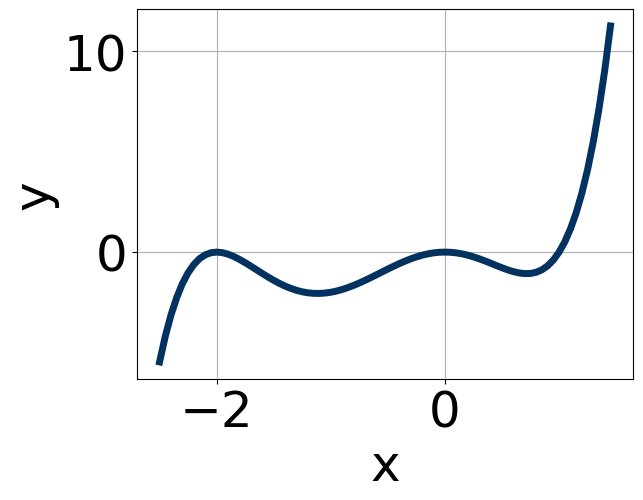
\includegraphics[width=0.5\textwidth]{../Figures/polyGraphToFunctionC.png}
\end{center}




The solution is \( 2x^{4} (x + 2)^{6} (x - 1)^{7} \), which is option A.\begin{enumerate}[label=\Alph*.]
\item \( 2x^{4} (x + 2)^{6} (x - 1)^{7} \)

* This is the correct option.
\item \( -20x^{6} (x + 2)^{8} (x - 1)^{7} \)

This corresponds to the leading coefficient being the opposite value than it should be.
\item \( -20x^{10} (x + 2)^{6} (x - 1)^{4} \)

The factor $(x - 1)$ should have an odd power and the leading coefficient should be the opposite sign.
\item \( 9x^{5} (x + 2)^{8} (x - 1)^{9} \)

The factor $x$ should have an even power.
\item \( 14x^{5} (x + 2)^{4} (x - 1)^{8} \)

The factor $x$ should have an even power and the factor $(x - 1)$ should have an odd power.
\end{enumerate}

\textbf{General Comment:} General Comments: Draw the x-axis to determine which zeros are touching (and so have even multiplicity) or cross (and have odd multiplicity).
}
\litem{
Describe the end behavior of the polynomial below.
\[ f(x) = -8(x + 8)^{5}(x - 8)^{6}(x - 2)^{2}(x + 2)^{3} \]

The solution is the graph below, which is option B.
\begin{center}
    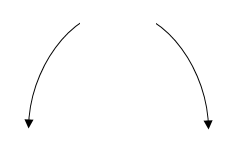
\includegraphics[width=0.3\textwidth]{../Figures/polyEndBehaviorCopyBC.png}
\end{center}\begin{enumerate}[label=\Alph*.]
\begin{multicols}{2}
\item 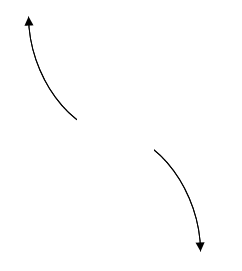
\includegraphics[width = 0.3\textwidth]{../Figures/polyEndBehaviorCopyAC.png}
\item 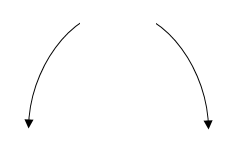
\includegraphics[width = 0.3\textwidth]{../Figures/polyEndBehaviorCopyBC.png}
\item 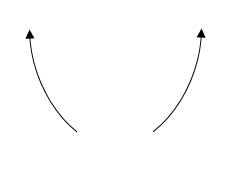
\includegraphics[width = 0.3\textwidth]{../Figures/polyEndBehaviorCopyCC.png}
\item 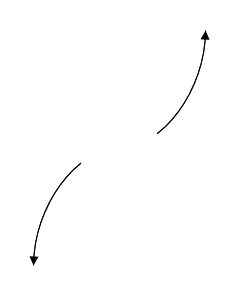
\includegraphics[width = 0.3\textwidth]{../Figures/polyEndBehaviorCopyDC.png}
\end{multicols}\item None of the above.\end{enumerate}
\textbf{General Comment:} Remember that end behavior is determined by the leading coefficient AND whether the \textbf{sum} of the multiplicities is positive or negative.
}
\litem{
Construct the lowest-degree polynomial given the zeros below. Then, choose the intervals that contain the coefficients of the polynomial in the form $ax^3+bx^2+cx+d$.
\[ \frac{2}{5}, \frac{1}{5}, \text{ and } 5 \]

The solution is \( 25x^{3} -140 x^{2} +77 x -10 \), which is option A.\begin{enumerate}[label=\Alph*.]
\item \( a \in [20, 28], b \in [-140, -132], c \in [71, 78], \text{ and } d \in [-17, -9] \)

* $25x^{3} -140 x^{2} +77 x -10$, which is the correct option.
\item \( a \in [20, 28], b \in [-111, -108], c \in [-73, -71], \text{ and } d \in [-17, -9] \)

$25x^{3} -110 x^{2} -73 x -10$, which corresponds to multiplying out $(5x + 2)(5x + 1)(x -5)$.
\item \( a \in [20, 28], b \in [-140, -132], c \in [71, 78], \text{ and } d \in [3, 13] \)

$25x^{3} -140 x^{2} +77 x + 10$, which corresponds to multiplying everything correctly except the constant term.
\item \( a \in [20, 28], b \in [137, 143], c \in [71, 78], \text{ and } d \in [3, 13] \)

$25x^{3} +140 x^{2} +77 x + 10$, which corresponds to multiplying out $(5x + 2)(5x + 1)(x + 5)$.
\item \( a \in [20, 28], b \in [-120, -116], c \in [-29, -19], \text{ and } d \in [3, 13] \)

$25x^{3} -120 x^{2} -27 x + 10$, which corresponds to multiplying out $(5x + 2)(5x -1)(x -5)$.
\end{enumerate}

\textbf{General Comment:} To construct the lowest-degree polynomial, you want to multiply out $(5x -2)(5x -1)(x -5)$
}
\litem{
Construct the lowest-degree polynomial given the zeros below. Then, choose the intervals that contain the coefficients of the polynomial in the form $x^3+bx^2+cx+d$.
\[ -5 + 5 i \text{ and } -2 \]

The solution is \( x^{3} +12 x^{2} +70 x + 100 \), which is option A.\begin{enumerate}[label=\Alph*.]
\item \( b \in [4, 22], c \in [68, 74], \text{ and } d \in [92, 107] \)

* $x^{3} +12 x^{2} +70 x + 100$, which is the correct option.
\item \( b \in [-1, 10], c \in [2, 12], \text{ and } d \in [9, 19] \)

$x^{3} + x^{2} +7 x + 10$, which corresponds to multiplying out $(x + 5)(x + 2)$.
\item \( b \in [-1, 10], c \in [-3, -1], \text{ and } d \in [-13, -9] \)

$x^{3} + x^{2} -3 x -10$, which corresponds to multiplying out $(x -5)(x + 2)$.
\item \( b \in [-13, -3], c \in [68, 74], \text{ and } d \in [-102, -96] \)

$x^{3} -12 x^{2} +70 x -100$, which corresponds to multiplying out $(x-(-5 + 5 i))(x-(-5 - 5 i))(x -2)$.
\item \( \text{None of the above.} \)

This corresponds to making an unanticipated error or not understanding how to use nonreal complex numbers to create the lowest-degree polynomial. If you chose this and are not sure what you did wrong, please contact the coordinator for help.
\end{enumerate}

\textbf{General Comment:} Remember that the conjugate of $a+bi$ is $a-bi$. Since these zeros always come in pairs, we need to multiply out $(x-(-5 + 5 i))(x-(-5 - 5 i))(x-(-2))$.
}
\litem{
Construct the lowest-degree polynomial given the zeros below. Then, choose the intervals that contain the coefficients of the polynomial in the form $ax^3+bx^2+cx+d$.
\[ \frac{3}{4}, -4, \text{ and } \frac{-2}{3} \]

The solution is \( 12x^{3} +47 x^{2} -10 x -24 \), which is option E.\begin{enumerate}[label=\Alph*.]
\item \( a \in [10, 16], b \in [-35, -30], c \in [-67, -55], \text{ and } d \in [-26, -22] \)

$12x^{3} -31 x^{2} -62 x -24$, which corresponds to multiplying out $(4x + 3)(x -4)(3x + 2)$.
\item \( a \in [10, 16], b \in [41, 52], c \in [-10, -6], \text{ and } d \in [24, 25] \)

$12x^{3} +47 x^{2} -10 x + 24$, which corresponds to multiplying everything correctly except the constant term.
\item \( a \in [10, 16], b \in [-48, -40], c \in [-10, -6], \text{ and } d \in [24, 25] \)

$12x^{3} -47 x^{2} -10 x + 24$, which corresponds to multiplying out $(4x + 3)(x -4)(3x -2)$.
\item \( a \in [10, 16], b \in [64, 69], c \in [72, 82], \text{ and } d \in [24, 25] \)

$12x^{3} +65 x^{2} +74 x + 24$, which corresponds to multiplying out $(4x + 3)(x + 4)(3x + 2)$.
\item \( a \in [10, 16], b \in [41, 52], c \in [-10, -6], \text{ and } d \in [-26, -22] \)

* $12x^{3} +47 x^{2} -10 x -24$, which is the correct option.
\end{enumerate}

\textbf{General Comment:} To construct the lowest-degree polynomial, you want to multiply out $(4x -3)(x + 4)(3x + 2)$
}
\end{enumerate}

\end{document}